\chapter[\cbalzeroshorttitle{}]{\cbalzerolongtitle{}}

\label{cbal0}

\section{Introduction, Definition, And History Of Boolean Algebra}
%Section tag:  INT0
\label{cbal0:sint0}

\index{Boolean algebra}
In this chapter, we review methods of 
simplifying \index{Boolean function}Boolean functions, and
show how such methods can be used to simplify software constructs
or to construct software which is more compact (in ROM or RAM) 
or executes more quicky.

Boolean algebra is named after \index{Boole, George}George Boole, 
a 19th-century British mathematician.
A fairly concise biography of George Boole comes from 
\cite{bibref:w:georgeboolebio01}:

\begin{quote}
George Boole first attended a school in Lincoln, then a commerical school.
His early instruction in mathematics, however, was from his father who
also gave George a liking for constructing optical instruments.  George's
interests turned to languages and he received instruction in Latin from a 
local bookseller.

By the age of 12 George had become so skilled in Latin that it provoked
an argument.  He translated an ode by the Latin poet Horace which his 
father was so proud of that he had it published.  However the talent was
such that a local schoolmaster disputed that any 12 year old could
have written with such depth.

Boole did not study for an academic degree, but from the age of 16 he was an 
assistant school teacher.  He maintained his interest in languages
and intended to enter the Church.  From 1835, however, he seems to have
changed his mind for he opened his own school and began to study mathematics
on his own.  He was later to realize that he had almost wasted five years
in trying to teach himself the subject instead of having a skilled teacher.

At this time Boole studied the works of Laplace and Lagrange, making 
notes which would later be the basis for his first mathematics paper.
However he did receive encouragement from Duncan Gregory who at this 
time was in Cambridge and the editor of the recently founded
\emph{Cambridge Mathematical Journal}.

Boole was unable to take Duncan Gregory's advice and study courses at 
Cambridge as he required the income from his school to look after
his parents.  However he began publishing in the \emph{Cambridge 
Mathematical Journal} and his interests were also influenced by Duncan Gregory
as he began to study algebra. An application of algebraic methods 
to the solution of differential equations was published by Boole in the
\emph{Transactions of the Royal Society} and for this work he received 
the Society's Royal Medal.  His mathematical work was beginning to bring
him fame.

Boole was appointed to the chair of mathematics at Queens College, 
Cork in 1849. He taught there for the rest of his life, gaining a reputation
as an outstanding and dedicated teacher.

In 1854 he published \emph{An investigation into the Laws of Thought, on 
Which are founded the Mathematical Theories of Logic and Probabilities}.
Boole approached logic in a new way reducing it to a simple algebra, 
incorporating logic into mathematics.  He pointed out the analogy
between algebraic symbols and those that represent logical forms. 
It began the algebra of logic called Boolean algebra which now finds
application in computer construction, switching circuits etc.

Boole also worked on differential equations, the influential 
\emph{Treatise on Differential Equations} appeared in 1859, the calculus of finite
differences, \emph{Treatise on the Calculus of Finite Differences} (1860), 
and general methods in probability. He published around 50 papers and
was one of the first to investigate the basic properties of numbers, such 
as the distributive property, that underlie the subject of algebra.

Many honours were given to Boole as the genius in his work was recognised. 
He received honorary degrees from the universities of Dublin
and Oxford and was elected a Fellow of the Royal Society (1857). 
However his career, which was started rather late, came to an unfortunately
early end when he died at the age of 49.  The circumstances are described 
by Macfarlane in [17]\footnote{As reproduced from 
\cite{bibref:w:georgeboolebio01}---this is not a valid reference
number in this work.} as follows:

\begin{quote}
One day in 1864 he walked from his residence to the College, 
a distance of two miles, in the drenching rain, and lectured in wet
clothes.  The result was a feverish cold which soon fell upon his 
lungs and terminated his career \ldots{}
\end{quote}

What Macfarlane fails to say is that Boole's wife 
(Mary---niece of Sir George Everest, after whom the mountain is named) believed that a
remedy should resemble the cause. She put Boole to bed and threw 
buckets of water over the bed since his illness had been caused by getting
wet.

Hirst described Boole as:

\begin{quote}
\ldots{} evidently an earnest able and at the same time a genial man.
\end{quote}

His work was praised by \index{DeMorgan, Augustus}De Morgan who said:

\begin{quote}
Boole's system of logic is but one of many proofs of genius and patience combined.
\ldots{} That the symbolic processes of algebra,
invented as tools of numerical calculation, should be competent to 
express every act of thought, and to furnish the grammar and
dictionary of an all-containing system of logic, would not have 
been believed until it was proved. When Hobbes \ldots{} published his
``Computation or Logique'' he had a remote glimpse of some of the points which 
are placed in the light of day by Mr Boole.
\end{quote}

Boolean algebra has wide applications in telephone switching and the 
design of modern computers. Boole's work has to be seen as a
fundamental step in today's computer revolution.
(Article by: J. J. O'Connor and E. F. Robertson.)
\end{quote}

In the preface of
\cite{bibref:b:whitesittbooleanalgandapps}, Whitesitt explains the
significance of Boole's work:

\begin{quote}
George Boole (1815-1864) introduced in his book \emph{The Laws Of Thought}
the first systematic treatment of logic and developed for this purpose
the algebraic system now known by his name, Boolean algebra.  Few
mathematical works of the last 100 years have had a greater impact
upon mathematics and philosophy than this famous book.  The significance
of the work has been well expressed by Augustus De Morgan:

\begin{quote}
That the symbolic processes of algebra, invented as tools of numerical
calculation, should be competent to express every act of thought, and to
furnish the grammar and dictionary of an all-containing system of
logic, would not have been believed until it was proved in
\emph{Laws Of Thought}.
\end{quote}

In addition to its applications in the field of logic, Boolean algebra
has two other important applications.  The first of these arises from
the fact that Boolean algebra is the natural algebra with which to
treat the combination of sets of elements under the operations of
intersection and union of sets.  With the addition of the idea of
``number of elements'' in a set, Boolean algebra becomes the 
foundation for the theory of probability.  The algebra
of sets is also important in many other branches of mathematics.

With the publication of two papers approximately 20 years 
ago,\footnote{Whitesitt's book was first published in 1961,
so Whitesitt probably means \emph{20 years ago} with 
respect to 1961.}
\index{Shannon, Claude E.}Claude E. Shannon introduced a new 
area of application of
Boolean algebra when he showed that the basic properties of
series and parallel combinations of bistable electrical
devices such as relays could be adequately represented
by this algebra.  Since this time, Boolean algebra has
played a significant role in the important and complicated
task of designing telephone switching circuits, automatic
control devices, and electronic computers.  At the present
time, more interest is centered in this application than
in either of the others.
\end{quote}

Claude E. Shannon's classic 1937 thesis is described separately
in several places.  From \cite{{bibref:w:boolealghist01}}:

\begin{quote}
Shannon, whose 1937 thesis centered on the improvement of the 
Differential Analyzer, a clunky mechanical gear and shaft addition
machine, realized that Boolean algebraic principles governed its operation.
He proposed that such a machine could be built with circuits using 
components that were governed by Boolean principles.  Shannon's paper
was regarded as genius and his ideas were almost immediately
incorporated into the telephone system.  Shannon took a position at Bell
Labs.  Later, of course, Shannon's thesis came to be seen as a focal point
in the development of modern computers.
\end{quote}

In \cite{bibref:w:boolealghist02}, Shannon's thesis is described
very favorably:

\begin{quote}
Around the 1850's, the British mathematician George Boole was 
busily inventing a new form of mathematics, in which he represented
logical expressions in a mathematical form now known as
Boolean Algebra.

Unfortunately, with the exception of students of philosophy
and symbolic logic, Boolean Algebra was destined to remain 
largely unknown and unused for the better part of a century.
It fact it was not until 1938 that Claude E. Shannon published
an article based on his master's thesis at MIT.  (Shannon's
thesis has since been described as: \emph{``Possibly the
most important master's thesis of the twentieth century.''})

In his paper, which was widely circulated, Shannon showed how
Boole's concepts of TRUE and FALSE could be used to represent
the functions of switches in electronic circuits.  It is difficult
to convey just how important this concept was; suffice it to say
that Shannon had provided electronics engineers with the mathematical
tool they needed to design digital electronic circuits, and these 
techniques remain the cornerstone of digital electronic
design to this day.

Apropos of nothing at all, Shannon is also credited with the invention
of the rocket-powered Frisbee, and is famous for riding down the
corridors of Bell Laboratories on a unicycle while simultaneously
juggling four balls.
\end{quote}

In summary, in 1854 George Boole published his classic work 
\emph{An investigation into the Laws of Thought, on 
Which are founded the Mathematical Theories of Logic and Probabilities},
which laid the foundation of manipulation of 
logical ideas using algebraic mechanisms.  Boole's ideas 
were revived in 1937 and 1938 by Claude E. Shannon
in his master's thesis and a subsequent article, in which
Shannon applied Boole's ideas to the design of electric
switching circuits.  Shannon's reapplication of Boole's work
came to be seen as a focal point in the development of modern
computers.


\section[Simplification By Algebraic Manipulation]
        {Simplification Of Boolean Functions By Algebraic Manipulation}
%Section Tag: SAM0
\label{cbal0:ssam0}

We assume that the reader has had previous exposure to 
\index{Boolean function!simplification of}simplification of
Boolean functions.  For this reason, this section is a review (it is terse
and moves quickly).  (For readers without this background, we
recommend \cite{bibref:b:manodigitaldesignseconded}.)

The most direct way to simplify Boolean functions is 
\index{Boolean function!algebraic simplification}\emph{algebraic}
transformation---to use transformation postulates and 
theorems to transform algebraic
expressions to a more desirable equivalent form.


\subsection{Nomenclature And Operators}
%Subsection Tag:  NOM0
\label{cbal0:ssam0:snom0}

We define the set of two elements which we will use in 
two-valued Boolean
algebra as `0' and '1' (or alternatively as 
`FALSE' and `TRUE', respectively).
All functions which we will describe subsequently require
inputs which are members of this set and will produce outputs
which are also members of this set.

The \emph{complement} or \emph{negation} operator (or function)
maps from 0$\rightarrow$1 and from 1$\rightarrow$0 (see Table 
\ref{tbl:cbal0:ssam0:snom0:01}).
We denote this operator
by an apostrophe
following the variable to be complemented (example: $x'$).
Alternatively, in some circumstances, we may use the
tilde ($\sim{}x$), the overbar ($\overline{x}$), or
the negation symbol ($\neg{}x$).

\begin{table}
\caption{Definition Of Logical Complement, Logical And, Logical Or, And Logical 
         Exclusive Or Operators}
\label{tbl:cbal0:ssam0:snom0:01}
\begin{center}
\begin{tabular}{|c|c||c|c|c|c|}
\hline
$X$ & $Y$  & $X'$ & $XY$ & $X+Y$ & $X \oplus{} Y$ \\
\hline
\hline
 0 & 0 & 1 & 0 & 0 & 0 \\
\hline
 0 & 1 & 1 & 0 & 1 & 1 \\
\hline
 1 & 0 & 0 & 0 & 1 & 1 \\
\hline
 1 & 1 & 0 & 1 & 1 & 0 \\
\hline
\end{tabular}
\end{center}
\end{table}

The \emph{logical AND} (or simply \index{AND}\index{Boolean algebra!AND}\emph{AND}) 
operator (or function)
returns TRUE if both of its input arguments are TRUE 
(see Table 
\ref{tbl:cbal0:ssam0:snom0:01}).
We denote this operator
by the \emph{times} symbol (example: $x \times{} y$), by
the keyword `AND', or by placing the operands adjacent to
each other (examples: $xy$, $x(y)$).

The \emph{logical OR}
(or simply \index{OR}\index{Boolean algebra!OR}\emph{OR}) 
operator (or function)
returns TRUE if either of its input arguments are TRUE 
(see Table 
\ref{tbl:cbal0:ssam0:snom0:01}).
We denote this operator
by the \emph{plus} symbol (example: $x + y$)  or by
the keyword `OR'.

The \emph{logical exclusive-OR}
(or simply \index{XOR}\index{Boolean algebra!XOR} \emph{XOR})
operator (or function)
returns TRUE if either but not both of its input arguments are TRUE 
(see Table 
\ref{tbl:cbal0:ssam0:snom0:01}).
We denote this operator
by the \emph{circled plus} symbol (example: $x \oplus{} y$),
by the \emph{caret} character (example: $x$\^{}$y$),  or by
the keyword `XOR'.

The exclusive-OR function is not a
function traditionally considered in the canonical forms of Boolean
algebra.  However, we consider it here because our aims may in
some cases be subtly
different than the aims of classic two-valued Boolean algebra.
The goal of classic Boolean algebra is to minimize the number of
terms which appear in a canonical form.
However, often our goal here is to rearrange Boolean functions into a form
which is optimal for implementation on a computer.  Since actual
computers usually provide a bitwise exclusive-OR instruction, there
are some applications where it may be useful to consider the
underlying instruction set of the computer (for example,
see \emph{Vertical Counters},
Section \ref{cbal0:svct0}).

In general, there are $2^{2^N}$ different Boolean functions of $N$
input variables, so it isn't practical to name functions involving more
than 2 input variables.  There are 16 ($=2^{2^2}$) Boolean functions of
2 input variables, and these are enumerated in
Table \ref{tbl:cbal0:ssam0:snom0:02}.

\begin{table}
\caption{Sixteen Possible Boolean Functions $f(A,B)$ Of Two Boolean Variables}
\label{tbl:cbal0:ssam0:snom0:02}
\begin{center}
\begin{tabular}{|c||c|c|c|c||l|}
\hline
\small{Func.} & $\scriptstyle{f(1,1)}$ & $\scriptstyle{f(1,0)}$ 
              & $\scriptstyle{f(0,1)}$ & $\scriptstyle{f(0,0)}$ 
			  & Function Description \\
\small{Num.}  &          &          &          &          &                 \\
\hline
\hline
 0 & 0 & 0 & 0 & 0 & \small{``Zero'' or  ``clear'' function.  Always}       \\
   &   &   &   &   & \small{returns zero regardless of $A$ and $B$  }       \\
   &   &   &   &   & \small{input values.                           }       \\
\hline
 1 & 0 & 0 & 0 & 1 & \small{Logical NOR = $(A+B)'$.                 }       \\
\hline
 2 & 0 & 0 & 1 & 0 & \small{Inhibition = $BA'$.  So named because   }       \\
   &   &   &   &   & \small{a TRUE value of $A$ inhibits $B$.  Also }       \\
   &   &   &   &   & \small{equivalent to $B>A$ or to $A<B$.        }       \\
\hline
 3 & 0 & 0 & 1 & 1 & \small{NOT A = $A'$.  Ignores $B$ and returns  }       \\
   &   &   &   &   & \small{$A'$.                                   }       \\
\hline
 4 & 0 & 1 & 0 & 0 & \small{Inhibition = $AB'$.  So named because   }       \\
   &   &   &   &   & \small{a TRUE value of $B$ inhibits $A$.  Also }       \\
   &   &   &   &   & \small{equivalent to $A>B$ or to $B<A$.        }       \\
\hline
 5 & 0 & 1 & 0 & 1 & \small{NOT B = $B'$.  Ignores $A$ and returns  }       \\
   &   &   &   &   & \small{$B'$.                                   }       \\
\hline
 6 & 0 & 1 & 1 & 0 & \small{Exclusive-OR (XOR) = $A \oplus B$.  Also}       \\
   &   &   &   &   & \small{equivalent to $A \neq B$.               }       \\
\hline
 7 & 0 & 1 & 1 & 1 & \small{Logical NAND = $(AB)'$.                 }       \\
\hline
 8 & 1 & 0 & 0 & 0 & \small{Logical AND = $AB$.                     }       \\
\hline
 9 & 1 & 0 & 0 & 1 & \small{Equivalence:  true if $A=B$.  Also}       \\
   &   &   &   &   & \small{known as exclusive-NOR, i.e. $(A \oplus B)'$.}       \\
\hline
10 & 1 & 0 & 1 & 0 & \small{Copy $B$.  Ignores $A$ and returns $B$. }       \\
\hline
11 & 1 & 0 & 1 & 1 & \small{Implication:  $B \rightarrow A$ (if $B$ }       \\
   &   &   &   &   & \small{then $A$).  Also equivalent to $B \geq A$.}     \\
\hline
12 & 1 & 1 & 0 & 0 & \small{Copy $A$.  Ignores $B$ and returns $A$. }       \\
\hline
13 & 1 & 1 & 0 & 1 & \small{Implication:  $A \rightarrow B$ (if $A$ }       \\
   &   &   &   &   & \small{then $B$).  Also equivalent to $A \geq B$.}     \\
\hline
14 & 1 & 1 & 1 & 0 & \small{Logical OR = $A+B$.                     }       \\
\hline
15 & 1 & 1 & 1 & 1 & \small{``One'' or ``set'' function.  Always    }       \\
   &   &   &   &   & \small{returns one regardless of $A$ and $B$   }       \\
   &   &   &   &   & \small{input values.                           }       \\
\hline
\end{tabular}
\end{center}
\end{table}

\emph{Any} Boolean function can be synthesized using AND gates and inverters
(i.e. NOT gates), OR gates and inverters, NAND gates alone, or NOR 
gates alone.  However, not all Boolean functions can be synthesized
using AND gates alone or OR gates alone.


\subsection{Postulates And Theorems}
%Subsection Tag:  POS0
\label{cbal0:ssam0:spos0}

Mathematicians tend to be very picky about what exactly a
\emph{postulate} is versus what a \emph{theorem} is.  We are
far less picky.  Either one (a postulate or a theorem) is a
rule that can be used to transform a Boolean algebraic expression
into another expression which is equivalent but for one reason or another
more desirable.  For our purposes here, postulates and theorems
are interchangeable.

Table \ref{tbl:cbal0:ssam0:spos0:01} 
(from \cite{bibref:b:manodigitaldesignseconded}) 
supplies the important postulates and theorems which are useful in
algebraically simplifying Boolean functions.

In Table \ref{tbl:cbal0:ssam0:spos0:01}, we should explain what 
is meant by the \emph{Dual Postulate Or Theorem}.  To
quote \cite{bibref:b:manodigitaldesignseconded}, p. 41:

\begin{quote}
\ldots This important property of Boolean algebra is called
the \index{Boolean algebra!duality principle}\index{duality principle}%
\emph{duality principle}.
It states that every algebraic expression deducible from the postulates
of Boolean algebra remains valid if the operators and identity
elements are interchanged.  In a two-valued Boolean algebra,
the identity elements and the elements of the set $B$ are the
same:  1 and 0.  The duality principle has many applications.
If the \emph{dual} of an algebraic expression is desired, we
simply interchange OR and AND operators and replaces 1s by
0s and 0s by 1s.
\end{quote}

\begin{table}
\caption{Important Postulates And Theorems Of Two-Valued Boolean Algebra}
\label{tbl:cbal0:ssam0:spos0:01}
\begin{center}
\begin{tabular}{|c||c|c||l|}
\hline
\small{Postulate} &  \small{Postulate}   & \small{Dual}        & \small{Remarks}   \\
\small{Or}        &  \small{Or}          & \small{Postulate}   &                   \\
\small{Theorem}   &  \small{Theorem}     & \small{Or}          &                   \\
\small{Number}    &                      & \small{Theorem}     &                   \\
\hline
      1           &  $x + 0 = x$         & $x \cdot 1 = 1$     &                   \\
\hline
      2           &  $x + x' = 1$        & $x \cdot x' = 0$    &                   \\
\hline
      3           &  $x + x = x$         & $x \cdot x = x$     &                   \\
\hline
      4           &  $x + 1 = 1$         & $x \cdot 0 = 0$     &                   \\
\hline
      5           &  $(x')' = x$         &                     & \small{Involution.} \\
\hline
      6           &  $x + y = y + x$     & $x \cdot y = y \cdot x $ & \small{Commutative property.} \\
\hline
      7           &  $x + (y + z)$       & $x(yz) = (xy)z$  & \small{Associative property.} \\
                  &  $= (x + y) + z$     &                     &                            \\
\hline
      8           &  $x (y + z)$         & $x + yz$          & \small{Distributive property.} \\
                  &  $= xy + xz$                    & $= (x+y)(x+z)$      &                                \\
\hline
      9           &  $(x+y)' = x'y'$      & $(xy)' = x' + y'$  & \small{DeMorgan's theorem.} \\
\hline
     10           &  $x + xy = x$         & $x(x+y) = x$       & \small{Absorption.} \\
\hline
\end{tabular}
\end{center}
\end{table}

Note also from Item 8 of
Table \ref{tbl:cbal0:ssam0:spos0:01} that in Boolean algebra
AND distributes over OR and OR distributes over AND (waiting on
newsgroup posters to clarify).  This is unlike ``normal'' algebra, where 
in general,

\begin{equation}
x + yz \neq (x+y) (x+z).
\end{equation}

The \index{Boolean algebra!operator precedence}%
\index{operator precedence!Boolean algebra}\index{operator precedence}%
operator precedence for evaluating Boolean expressions assumed throughout
this work is:

\begin{quote}
\begin{enumerate}
\item Parenthesis.
\item NOT.
\item AND.
\item OR.
\end{enumerate}
\end{quote}

\noindent{}Note that this operator precedence very closely mirrors
the standard precedence of normal algebraic expressions.

\subsection{Canonical And Standard Forms}
%Subsection Tag:  CAS0
\label{cbal0:ssam0:scas0}

\cite{bibref:b:manodigitaldesignseconded}, p. 49 provides an concise and
excellent definition of \emph{minterms} and \emph{maxterms}.  The definition
here is taken primarily from that source.

A binary variable may appear either in its normal form ($x$, for example)
or in its complemented form ($x'$, for example).  Now consider two
binary variables $x$ and $y$ combined with an AND
operation.  Since each variable may appear in either form, there are four
possible combinations:  $x'y'$, $x'y$, $xy'$, and $xy$.  These
four AND terms are mutually exclusive and mutually exhaustive---that is,
no combination of values for
$x$ and
$y$ that causes one of these AND terms to be TRUE may cause any of the
others to be TRUE, and every combination of $x$ and $y$ will cause exactly
one of these AND terms to be TRUE.  Each of these
four AND terms is called a \index{Boolean algebra!minterm}\index{minterm}\emph{minterm}
or \index{Boolean algebra!standard product}\index{standard product}\emph{standard product}.
In a similar manner, $n$ variables can be combined to form $2^n$ minterms.

In a similar fashion, $n$ variables forming an OR term, with each variable 
being primed or unprimed, provide $2^n$ possible combinations, called
\index{Boolean algebra!maxterm}\index{maxterm}\emph{maxterms}, or
\index{Boolean algebra!standard sum}\index{standard sum}\emph{standard sums}.

\begin{table}
\caption{Minterms And Maxterms Of Three Boolean Variables}
\label{tbl:cbal0:ssam0:scas0:01}
\begin{center}
\begin{tabular}{|c|c|c||c|c||c|c|}
\hline
 $x$ & $y$ & $z$ & \small{Minterm} &  \small{Minterm}     & \small{Maxterm} & \small{Maxterm}     \\
     &     &     & \small{Term}    &  \small{Designation} & \small{Term}    & \small{Designation} \\
\hline
  0  &  0  &  0  & $x'y'z'$        &  $m_0$               & $x+y+z$         & $M_0$               \\
\hline
  0  &  0  &  1  & $x'y'z$         &  $m_1$               & $x+y+z'$        & $M_1$               \\
\hline
  0  &  1  &  0  & $x'yz'$         &  $m_2$               & $x+y'+z$        & $M_2$               \\
\hline
  0  &  1  &  1  & $x'yz$          &  $m_3$               & $x+y'+z'$       & $M_3$               \\
\hline
  1  &  0  &  0  & $xy'z'$         &  $m_4$               & $x'+y+z$        & $M_4$               \\
\hline
  0  &  0  &  1  & $x'y'z$         &  $m_5$               & $x+y+z'$        & $M_5$               \\
\hline
  1  &  1  &  0  & $xyz'$          &  $m_6$               & $x'+y'+z$       & $M_6$               \\
\hline
  1  &  1  &  1  & $xyz$           &  $m_7$               & $x'+y'+z'$      & $M_7$               \\
\hline
\end{tabular}
\end{center}
\end{table}

The two primary canonical forms in Boolean algebra are the
\emph{sum of minterms} (or \emph{sum of products}) form and the
\emph{product of maxterms} (or \emph{product of sums}) form.

The sum of minterms canonical form (which is the most common
canonical form) is sometimes written using a shorthand 
notation involving the Greek letter sigma ($\Sigma$).  We describe this
shorthand form now.  Consider the Boolean function of 3 variables,

\begin{equation}
\label{eq:cbal0:ssam0:scas0:01}
F(A, B, C) = A + B'C.
\end{equation}

\noindent{}Using the postulates and theorems in Table 
\ref{tbl:cbal0:ssam0:spos0:01}, it is possible
to expand (\ref{eq:cbal0:ssam0:scas0:01}) into
a sum of minterms form:

\begin{eqnarray}
\label{eq:cbal0:ssam0:scas0:02}
F(A, B, C) & = & A'B'C + AB'C' + AB'C + ABC' + ABC \\
           & = & m_1 m_4 m_5 m_6 m_7.\nonumber
\end{eqnarray}

\noindent{}(\ref{eq:cbal0:ssam0:scas0:02}) is also commonly written
in the shorthand form:

\begin{equation}
\label{eq:cbal0:ssam0:scas0:03}
F(A, B, C) = \Sigma{}(1, 4, 5, 6, 7).
\end{equation}

\noindent{}In the right-hand side of
(\ref{eq:cbal0:ssam0:scas0:03}), each integer
(1, 4, 5, 6, or 7) corresponds to the integer
that would be formed by treating the corresponding
minterm in (\ref{eq:cbal0:ssam0:scas0:02}) as
a binary number, i.e. $A=2^2$, $B=2^1$, and
$C=2^0$.  This is the basis of the short hand
notation.

A second but much less commonly used canonical form
is the product of maxterms (or product of sums) form,
which uses the Greek letter pi ($\Pi$) for its shorthand
form.  Without further explanation, we present the 
product of maxterms form of $\Sigma{}(1,4,5,6,7)$
(Eqns. \ref{eq:cbal0:ssam0:scas0:01} through
\ref{eq:cbal0:ssam0:scas0:03}) as
(\ref{eq:cbal0:ssam0:scas0:04}) 
through (\ref{eq:cbal0:ssam0:scas0:07}) 
(Figure \ref{fig:cbal0:ssam0:scas0:01}).

\begin{figure}
\begin{eqnarray}
\label{eq:cbal0:ssam0:scas0:04}
F(A, B, C) & = & \Sigma{}(1, 4, 5, 6, 7) \\
\label{eq:cbal0:ssam0:scas0:05}
           & = & \Pi{}(0, 2, 3)          \\
\label{eq:cbal0:ssam0:scas0:06}
		   & = & M_0 M_2 M_3             \\
\label{eq:cbal0:ssam0:scas0:07}
		   & = & (x+y+z)(x+y'+z)(x+y'+z')
\end{eqnarray}
\caption{Product Of Maxterms Form Of $\Sigma{}(1,4,5,6,7)$}
\label{fig:cbal0:ssam0:scas0:01}
\end{figure}


Because there are so many excellent digital logic books on the market
that contain examples and exercises of algebraic simplification
(we recommend \cite{bibref:b:manodigitaldesignseconded}), we don't
dwell on algebraic simplification or provide examples.  Again, we
assume that nearly all of our readers have had a course in digital
logic or symbolic logic.


\section[Karnaugh Maps]
        {Simplification Of Boolean Functions Using Karnaugh Maps}
%Section tag:  SKM0
\label{cbal0:skm0}

In 1953, M. Karnaugh published the graphical map method of simplifying
combinational logic functions (\cite{bibref:p:kmapclassic01}).  This
method has come to be known as the \emph{Karnaugh map} or \emph{K-map}
method of reduction, and is taught to engineers in nearly every
digital logic class.

Although it is possible, starting from an arbitrary Boolean formula, to simplify
the formula through algebraic manipulation, algebraic simplification
has the disadvantage that formulas can have many forms and there is not
an easily remembered, precise, and repeatable procedure for algebraic simplification.
The Karnaugh map method has the advantage that each Boolean function
has only one graphical representation, and that the procedure for simplification
is simple and easily remembered.

In a Karnaugh map, each square corresponds to a possible minterm of the function.
The essence of the method is to populate a grid of squares with outputs of
the function to be simplified.  Each minterm that must exist in the
function (i.e. each combination of inputs for which the function
must return TRUE) receives a `1' in the corresponding square.  Each
combination of inputs for which the function must return FALSE
receives a `0' in the corresponding square.  Each combination of inputs
for which the function may return either TRUE or FALSE receives an
`X' in the corresponding square.

After the Karnaugh map squares are populated with 1's, 0's, and X's
corresponding to the required values of the function for each combination
of inputs, the 1's are graphically combined into the largest rectangle possible.
Each rectangle may include 1's, may include X's where convenient, but
may not include 0's.
Each of these squares is then translated into a product of uncomplemented and
complemented input variables, and these products are summed to
produce the simplified algebraic expression for the function.  (We don't 
belabor this process, because we assume that most of our readers
understand it very thoroughly.)  There are some subtle points
to the process, such as combining corners and the ``folding'' of the
5- and 6-variable maps, but we don't explain these subtle points here
because they are so thoroughly explained in so many books.

Figures \ref{fig:cbal0:skm0:00} through \ref{fig:cbal0:skm0:04}
supply the canonical forms of two-, three-, four-, five-, and
six-variable Karnaugh maps.

\begin{figure}
\centering
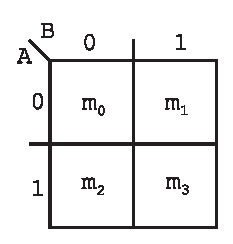
\includegraphics[width=1.25in]{c_bal0/kmap02cf.eps}
\caption{Canonical Form Of Two-Variable Karnaugh Map}
\label{fig:cbal0:skm0:00}
\end{figure}

\begin{figure}
\centering
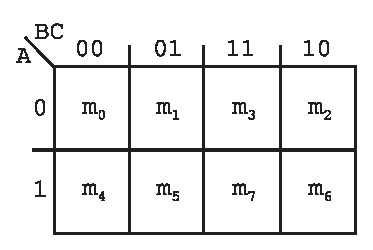
\includegraphics[height=1.25in]{c_bal0/kmap03cf.eps}
\caption{Canonical Form Of Three-Variable Karnaugh Map}
\label{fig:cbal0:skm0:01}
\end{figure}

\begin{figure}
\centering
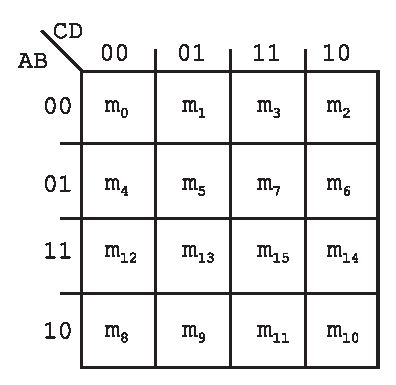
\includegraphics[height=2.0in]{c_bal0/kmap04cf.eps}
\caption{Canonical Form Of Four-Variable Karnaugh Map}
\label{fig:cbal0:skm0:02}
\end{figure}

\begin{figure}
\centering
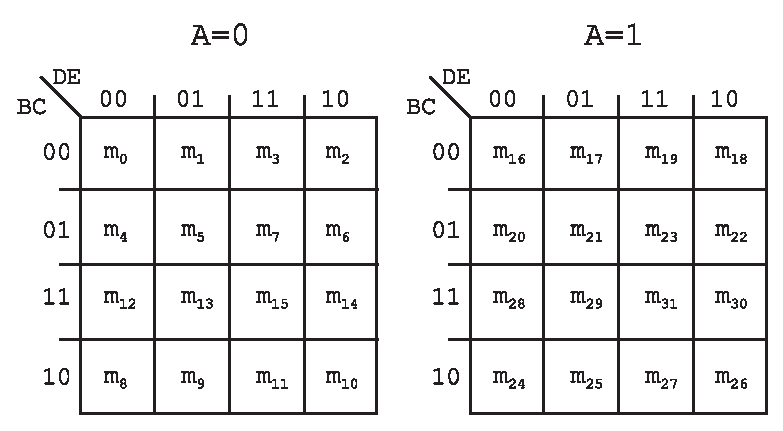
\includegraphics[width=4.25in]{c_bal0/kmap05cf.eps}
\caption{Canonical Form Of Five-Variable Karnaugh Map}
\label{fig:cbal0:skm0:03}
\end{figure}

\begin{figure}
\centering
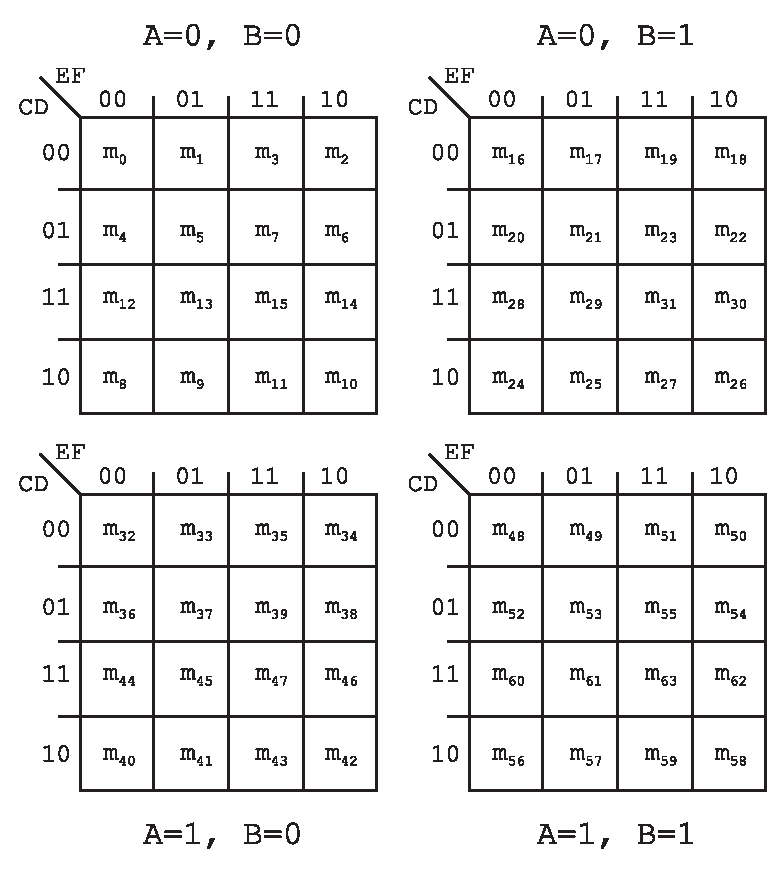
\includegraphics[width=4.5in]{c_bal0/kmap06cf.eps}
\caption{Canonical Form Of Six-Variable Karnaugh Map}
\label{fig:cbal0:skm0:04}
\end{figure}

\section[Simplification Using The Scheinman Method]
        {Simplification Of Boolean Functions Using The Scheinman Method}
%Section Tag: SCM0
\label{cbal0:sscm0}

Two major disadvantages of the Karnaugh map method of simplifying Boolean
functions are that:

\begin{itemize}
\item It is generally not possible to apply the method to functions
      of more than six variables.
\item It is not easy to automate the method (in the form that it is stated)
      because it is inherently graphical.
\end{itemize}

In 1962, A. H. Scheinman published a method for the simplification
of Boolean functions (\cite{bibref:p:scheinmanclassic01}) which is more amenable
to automation than the Karnaugh map method.

\section[The Quine-McCluskey Method]
        {Simplification Of Boolean Functions Using The Quine-McCluskey Method}


\section{Multiple Functions Of $N$ Boolean Variables}

Need to get back to Dr. Singh to inquire about the multiple Scheinman method.

\section{Vertical Counters}
%Section Tag: VCT0.
\label{cbal0:svct0}

\index{vertical counter}As has been hinted at elsewhere 
in this work, the need to generate
firmware which minimizes ROM consumption leads to clever (but perhaps
less-than-intuitive) programming techniques.  One such technique
is the construction of \emph{vertical counters}.  

A \index{vertical counter}vertical counter
is a set of identical combinational mappings or state machines 
where the inputs, state vector, intermediate results, and outputs of each
combinational mapping or state machine are stored as a single bit 
in the same position 
in each of multiple bytes or words.  When inputs, state vectors,
intermediate results, and outputs are stored
in this way, the bitwise logical instructions of the machine
(AND, OR, NOT, XOR) can be used to process several state machines in
parallel.  Vertical counters are intimately related to the reduction
of Boolean functions because such reduction must be performed in order
to design the vertical counter.  Debouncing and filtering, where the 
inputs and outputs naturally tend to be arranged as groups of bits,
are the most common application of vertical counters.

A very helpful resource on the web is the set of web pages 
maintained by \index{Dattalo, Scott}Scott Dattalo 
\cite{bibref:i:scottdattalo} for the
PIC microcontroller, including
especially \cite{bibref:w:sdattalovc02}.  Many of the vertical counter
designs which follow come from Mr. Dattalo's pages.

We abuse the term \emph{counter} somewhat, and we refer to 
any bit-wise mapping useful in microcontroller work as
a vertical counter.  We categorize vertical counters as 
\index{vertical counter!combinational}\emph{combinational}
(not truly a counter---the output is a function of the
inputs only), \index{vertical counter!sequential}\emph{sequential}
(the next state and output may be functions of both the
inputs and the present state---i.e. a proper state machine),
\index{vertical counter!cyclic}\emph{cyclic} (the counter
goes through a series of states and then repeats), or
\index{vertical counter!terminating} (the counter 
will reach a terminal state).

\subsection{2-Bit 4-State Cyclic Vertical Counter}
%Subsection Tag: TBF0
\label{cbal0:svct0:stbf0}
In this discussion of vertical counters, we begin with the simplest
designs, as often the simpler designs appear as part of more complex
designs.

Table \ref{tbl:cbal0:svct0:stbf0:01} supplies the state transition table 
for a 2-bit 4-state
cyclic vertical counter.  Note that the counter advances through the
bit patterns in the ``proper'' binary integer order.

\begin{table}
\caption{State Transition Table Of 2-Bit 4-State Cyclic Vertical Counter}
\label{tbl:cbal0:svct0:stbf0:01}
\begin{center}
\begin{tabular}{|c|c|c|c|}
\hline
 $A_k$     & $B_k$     & $A_{k+1}$ & $B_{k+1}$ \\
\hline
\hline
 0         & 0         & 0         & 1         \\
\hline
 0         & 1         & 1         & 0         \\
\hline
 1         & 0         & 1         & 1         \\
\hline
 1         & 1         & 0         & 0         \\
\hline
\end{tabular}
\end{center}
\end{table}

From Table \ref{tbl:cbal0:svct0:stbf0:01} it can be readily verified
even without a Karnaugh map that the least significant bit
($B$) is always complemented from one state to the next, so that
$B_{k+1} = \neg B_k$.  It can also be seen that the most significant
bit ($A$) is complemented from one state to the next only if $B$=1,
so that $A_{k+1} = A_k \oplus B_k$.

The implementation of such a counter in `C' comes immediately, since
`C' directly supports bit-wise complementation and exclusive-OR of
integers:

\begin{verbatim}
         A = A ^ B;
         B = ~B;
\end{verbatim}

Note in the `C' snippet above, the two operations are ordered so as
not to interfere with each other.  Note that reversing the two steps above
would not yield the desired result.


\subsection{3-Bit 8-State Cyclic Vertical Counter}
%Subsection Tag: TBF4
\label{cbal0:svct0:stbf4}


\subsection[$N$-Bit $2^N$-State Cyclic Vertical Counter]
           {\mbox{\boldmath $N$}-Bit \mbox{\boldmath $2^N$}-State Cyclic Vertical Counter}
%Subsection Tag: TBF1
\label{cbal0:svct0:stbf1}

The design of the 2-bit 4-state vertical counter presented in
Section \ref{cbal0:svct0:stbf0} (immediately above) and be
generalized to an $N$-bit $2^N$-state counter which follows
the traditional binary integer counting sequence.

Note from Section \ref{cbal0:svct0:stbf0} that the least
significant bit of the counter is always complemented
in going from one state to the next, and that each more
significant bit is complemented only if all less significant 
bits are 1.  If $X_0$ is the least significant bit of the 
counter and $X_N$ the most significant bit,
(\ref{eq:cbal0:svct0:stbf1:01}) through (\ref{eq:cbal0:svct0:stbf1:05})
(Figure \ref{eq:cbal0:svct0:stbf1:01})
describe how the counter is advanced from one state to the next.
Note that this set of equations gives only a \emph{logical} description
of how to obtain the next state from the present state---these
equations cannot be used as a direct blueprint for implementation because
earlier steps would destroy the results needed for later steps.

\begin{figure}
\begin{eqnarray}
\label{eq:cbal0:svct0:stbf1:01}
  X_0(k+1) & = & \neg X_0(k)                             \\
\label{eq:cbal0:svct0:stbf1:02}
  X_1(k+1) & = & X_1(k) \oplus X_0(k)                    \\ 
\label{eq:cbal0:svct0:stbf1:03}
  X_2(k+1) & = & X_2(k) \oplus (X_1(k) X_0(k))           \\
\label{eq:cbal0:svct0:stbf1:04}
  X_3(k+1) & = & X_3(k) \oplus (X_2(k) X_1(k) X_0(k))    \\
           & \ldots & \nonumber                          \\
\label{eq:cbal0:svct0:stbf1:05}
  X_N(k+1) & = & X_N(k) \oplus (X_{N-1}(k) \ldots X_0(k))
\end{eqnarray}
\caption{State Transition Equations Of $N$-Bit $2^N$-State Cyclic Vertical Counter}
\label{fig:cbal0:svct0:stbf1:01}
\end{figure}

The form of 
(\ref{eq:cbal0:svct0:stbf1:01}) through (\ref{eq:cbal0:svct0:stbf1:05})
suggests a way to economically implement an $N$-bit $2^N$-state
cyclic vertical counter in software, using two temporary
variables $TEMP_A$ and $TEMP_B$.  The general blueprint for
implementation is supplied as
(\ref{eq:cbal0:svct0:stbf1:06}) through (\ref{eq:cbal0:svct0:stbf1:20})
(Figure \ref{eq:cbal0:svct0:stbf1:02}).

\begin{figure}
\begin{eqnarray}
\label{eq:cbal0:svct0:stbf1:06}
  TEMP_A   & = & X_0                                     \\
\label{eq:cbal0:svct0:stbf1:07}
  X_0      & = & \neg X_0                                \\
\label{eq:cbal0:svct0:stbf1:08}
  TEMP_B   & = & X_1 TEMP_A                              \\
\label{eq:cbal0:svct0:stbf1:09}
  X_1      & = & X_1 \oplus TEMP_A                       \\ 
\label{eq:cbal0:svct0:stbf1:10}
  TEMP_A   & = & TEMP_B                                  \\
\label{eq:cbal0:svct0:stbf1:11}
  TEMP_B   & = & X_2 TEMP_B                              \\
\label{eq:cbal0:svct0:stbf1:12}
  X_2      & = & X_2 \oplus TEMP_A                       \\
\label{eq:cbal0:svct0:stbf1:13}
  TEMP_A   & = & TEMP_B                                  \\
\label{eq:cbal0:svct0:stbf1:14}
  TEMP_B   & = & X_3 TEMP_B                              \\
\label{eq:cbal0:svct0:stbf1:15}
  X_3      & = & X_3 \oplus TEMP_A                       \\
           & \ldots & \nonumber                          \\
\label{eq:cbal0:svct0:stbf1:16}
  X_{N-2}  & = & X_{N-2} \oplus TEMP_A                   \\
\label{eq:cbal0:svct0:stbf1:17}
  TEMP_A   & = & TEMP_B                                  \\
\label{eq:cbal0:svct0:stbf1:18}
  TEMP_B   & = & X_{N-1} TEMP_B                          \\
\label{eq:cbal0:svct0:stbf1:19}
  X_{N-1}  & = & X_{N-1} \oplus TEMP_A                   \\
\label{eq:cbal0:svct0:stbf1:20}
  X_N      & = & X_N \oplus X_N TEMP_B
\end{eqnarray}
\caption{Implementation Blueprint Of $N$-Bit $2^N$-State Cyclic Vertical Counter}
\label{fig:cbal0:svct0:stbf1:02}
\end{figure}

Figure \ref{fig:cbal0:svct0:stbf1:01} 
supplies a concrete example of a C-language
implementation of a 5-bit 32-state cyclic vertical counter.
Note that the counter will follow the traditional 
binary integer counting sequence.  Note also that
the blueprint provided by Eqns. 
(\ref{eq:cbal0:svct0:stbf1:06}) through (\ref{eq:cbal0:svct0:stbf1:20})
and Figure \ref{fig:cbal0:svct0:stbf1:01} can 
be extended to a counter of any size.

\begin{figure}
\begin{verbatim}
/**************************************************************/
/* Assume:                                                    */
/*    x4     : Byte containing most significant bits of the   */
/*             a group of 8 bits.                             */
/*    x3,                                                     */
/*    x2,                                                     */
/*    x1     : Bytes containing the intermediate bits.        */
/*    x0     : Byte containing the least significant bits.    */
/*    temp_a,                                                 */
/*    temp_b : Temporary variables, used to accumulate the    */
/*             result of AND'ing old counter bit values.      */
/**************************************************************/

temp_a =  x0;
x0     = ~x0;
temp_b =  x1 & temp_a;
x1     =  x1 ^ temp_a;
temp_a =  temp_b;
temp_b =  x2 & temp_b;
x2     =  x2 ^ temp_a;
temp_a =  temp_b;
temp_b =  x3 & temp_b;
x3     =  x3 ^ temp_a;
x4     =  x4 ^ temp_b;

/* End of code. */
\end{verbatim}
\caption{C-Language Implementation Of 5-Bit 32-State Cyclic Vertical Counter}
\label{fig:cbal0:svct0:stbf1:01b}
\end{figure}


\subsection{3-Bit 5-State Cyclic Vertical Counter}
%Subsection Tag: TBF5
\label{cbal0:svct0:stbf5}


\subsection{3-Bit 6-State Cyclic Vertical Counter}
%Subsection Tag: TBF6
\label{cbal0:svct0:stbf6}


\subsection{3-Bit 7-State Cyclic Vertical Counter}
%Subsection Tag: TBF7
\label{cbal0:svct0:stbf7}


\subsection{2-Bit 4-State Terminating Vertical Counter}
%Subsection Tag: TBF8
\label{cbal0:svct0:stbf8}


\subsection{3-Bit 5-State Terminating Vertical Counter}
%Subsection Tag: TBF9
\label{cbal0:svct0:stbf9}


\subsection{3-Bit 6-State Terminating Vertical Counter}
%Subsection Tag: TBG0
\label{cbal0:svct0:stbg0}


\subsection{3-Bit 7-State Terminating Vertical Counter}
%Subsection Tag: TBG1
\label{cbal0:svct0:stbg1}


\subsection{2/3 Debouncing Vertical Counter}
%Subsection Tag: TTD0.
\label{cbal0:svct0:sttd0}

\index{debouncing}\index{debouncing!2/3}\emph{2/3 debouncing} 
is debouncing where at least two of the most recent
three samples must be at the same value (either 0 or 1) to cause the output
to be that same value.

Note that \emph{2/3 debouncing} as we describe it here represents a
purely combinational mapping from the 3 most recent samples to
the debounced output.  When 3 samples are available, 0 of the
samples or 1 of the samples with value 1 map to a debounced
output value of 0; while 2 of the samples or 3 of the samples
with value 1 map to a debounced output value of 1.

If $A$ is the most recent sample, $B$ is the next-most-recent sample, and 
$C$ is the oldest sample, Fig. \ref{fig:cbal0:svct0:sttd0:01} 
supplies the Karnaugh map for 2/3
debouncing.

\begin{figure}
\centering
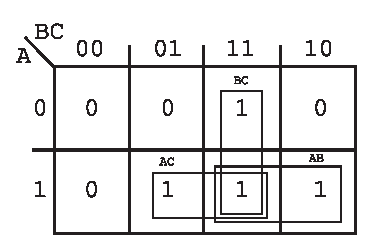
\includegraphics[height=1.25in]{c_bal0/kmap23db.eps}
\caption{Karnaugh Map Of 2/3 Debouncing}
\label{fig:cbal0:svct0:sttd0:01}
\end{figure}

It can be seen from the figure that the expression for the output is

\begin{equation}
\label{eq:cbal0:svct0:sttd0:01}
AB + AC + BC = A (B+C) + BC .
\end{equation}

Intuitively, (\ref{eq:cbal0:svct0:sttd0:01}) makes sense---the output 
will be 1 if any two of the most recent samples are 1
($AB + AC + BC$).  Similarly, the output will be 0 if any two of
the most recent samples are 0.

Figure \ref{fig:cbal0:svct0:sttd0:02} supplies the C-language
code to implement 2/3 debouncing as a vertical mapping.
A C-compiler will typically implement this code very directly
using the bitwise logical instructions of the machine.

\begin{figure}
\begin{verbatim}
/**************************************************************/
/* Assume:                                                    */
/*    A      : Most recent sample (i.e. at t(0)), arranged as */
/*             a group of 8 bits.                             */
/*    B      : Next most recent sample t(-1).                 */
/*    C      : Oldest sample t(-2).                           */
/*    output : Debounced collection of 8 bits presented to    */
/*             software internals.                            */
/**************************************************************/

output = (A & (B | C)) | (B & C);

/* End of code. */
\end{verbatim}
\caption{C-Language Implementation Of 2/3 Debouncing}
\label{fig:cbal0:svct0:sttd0:02}
\end{figure}

\subsection{3/3 Debouncing Vertical Counter}
%Subsection Tag: TTD1.
\label{cbal0:svct0:sttd1}

\index{debouncing}\index{debouncing!3/3}\emph{3/3 debouncing} 
is debouncing where all three of the most recent
three samples must be at a value (either 0 or 1) to cause the 
debounced output to transition to that same value.

Note that 3/3 debouncing as we present it is a sequential (rather than
a purely combinational) mapping from the 3 most recent samples to the
debounced output.  In addition to the 3 inputs, the behavior of the
mapping depends on a single bit of state which is held.  (In the
implementation presented in this section, the state and the debounced
output are the same bit.)  For example, if 2 of the 3 most recent
input samples are 1, the debounced output value may be either 0
or 1.  The transition of the debounced output value from
0 to 1 or from 1 to 0 can only occur if all 3 most recent samples
are 1 or are 0, respectively.

If $A$ is the most recent sample, $B$ is the next-most-recent sample,
$C$ is the oldest sample, and $O$ is the output (assumed maintained
as a RAM location) Fig. \ref{fig:cbal0:svct0:sttd1:01} 
supplies the Karnaugh map for 3/3
debouncing.

\begin{figure}
\centering
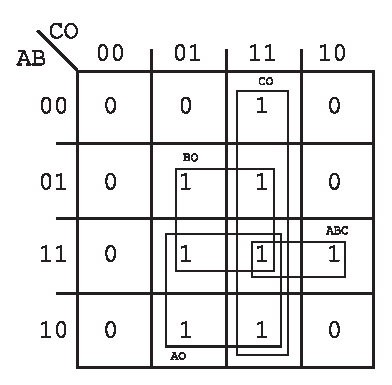
\includegraphics[height=2.0in]{c_bal0/kmap33db.eps}
\caption{Karnaugh Map Of 3/3 Debouncing}
\label{fig:cbal0:svct0:sttd1:01}
\end{figure}

It can be seen from the figure that the expression for the output is

\begin{equation}
\label{eq:cbal0:svct0:sttd1:01}
ABC + AO + BO + CO = ABC + O(A + B + C).
\end{equation}

Intuitively, (\ref{eq:cbal0:svct0:sttd1:01}) makes sense---the output 
will be unconditionally 1 if all three of the most recent samples are 1
($ABC$).  The output will also be 1 if the previous output was 1
and at least one of the most recent samples are 1 [$O(A+B+C)$]---at least
one true recent sample blocks the output from transition to 0.

Figure \ref{fig:cbal0:svct0:sttd1:02} supplies the C-language
code to implement 3/3 debouncing as a vertical mapping.
A C-compiler will typically implement this code very directly
using the bitwise logical instructions of the machine.

\begin{figure}
\begin{verbatim}
/**************************************************************/
/* Assume:                                                    */
/*    A      : Most recent sample (i.e. at t(0)), arranged as */
/*             a group of 8 bits.                             */
/*    B      : Next most recent sample t(-1).                 */
/*    C      : Oldest sample t(-2).                           */
/*    output : Debounced collection of 8 bits presented to    */
/*             software internals.  Note that this is both    */
/*             an input (to the combinational mapping) and    */
/*             the new result.                                */
/**************************************************************/

output = (A & B & C) | (output & (A | B | C));

/* End of code. */
\end{verbatim}
\caption{C-Language Implementation Of 3/3 Debouncing}
\label{fig:cbal0:svct0:sttd1:02}
\end{figure}

\subsection{N/N Debouncing Vertical Counter}
%Subsection Tag: NNC0.
\label{cbal0:svct0:snnc0}

\index{debouncing}\index{debouncing!N/N}It is clear from 
the design of the 3/3 debouncing
vertical counter (Section \ref{cbal0:svct0:sttd1}, immediately
above) that the design of the 3/3 debouncing vertical counter
can be generalized to cover any number of recent samples.
We call such a debouncing vertical counter an N/N debouncing
vertical counter.  In order for the output of such a counter to
turn 1, all $N$ most recent samples must be 1.  Similarly, in order
for such a counter to turn 0, all $N$ most recent samples must be 0.

We rely on a logical argument to design such a N/N debouncing
vertical counter, rather than on Karnaugh maps.  If $I_1 \ldots I_N$
are the $N$ most recent input samples and $O$ is the most recent
output (assumed stored in RAM), it is clear from the form of
(\ref{eq:cbal0:svct0:sttd1:01}) that the formula for the new output
as a function of the inputs $I_1 \ldots I_N$ and the 
most recent output $O_{k-1}$ must be:

\begin{equation}
\label{eq:cbal0:svct0:snnc0:01}
O_k = I_1 I_2 \ldots I_N + (O_{k-1} (I_1 + I_2 + \ldots + I_N)) .
\end{equation}

The form of (\ref{eq:cbal0:svct0:snnc0:01}) is intuitively 
plausible.  If the previous output $O_{k-1}$ is 0, the only
circumstance under which the next output $O_k$ will become 1
is if all $N$ inputs $I_1, I_2, \ldots , I_N$ are 1.
Similarly, if the previous output $O_{k-1}$ is 1, the only
circumstance under which $O_k$ will become 0
is if all $N$ inputs $I_1, I_2, \ldots , I_N$ are 0.  This
is the desired behavior.

For an N/N counter when a large number of previous samples
are required to be at the same value (say, $N=10$, for example),
it may seem that the efficiency of the N/N vertical counter
design presented here will break down.  However, it must be
remembered that the vertical counter approach manipulates
a large number (usually 8 or 16) inputs at a time.  It can be
shown easily that an N/N debouncing vertical counter requires
$2N$ operations to determine the next output.  Thus, for a
10/10 debouncing vertical counter, the necessary software 
may execute in as little as 20 machine instructions.  It would
be difficult to find another method which will perform 10/10
debouncing for 8 or 16 inputs in only 20 machine instructions, thus
we maintain that the N/N debouncing vertical counter
approach presented is quite efficient even for larger
$N$.


\section{Authors And Acknowledgements}
%Section tag:  ACK0
This chapter was primarily written by David T. Ashley
\cite{bibref:i:daveashley}.

We are very grateful to \index{Dattalo, Scott}Scott Dattalo 
\cite{bibref:i:scottdattalo},
whose web pages about vertical counters provided much of the
material for the Section \ref{cbal0:svct0}.
Special thanks to \index{Virgil}Virgil \cite{bibref:i:virgil},
\index{Dresner, Norm}Norm Dresner \cite{bibref:i:normdresner},
and \index{Kaskelma, Heikki}Heikki Kaskelma \cite{bibref:i:heikkikaskelma}
for mathematical assistance provided via the 
\index{sci.math newsgroup@\texttt{sci.math} newsgroup}%
\texttt{sci.math} \cite{bibref:n:scimathnewsgroup} newsgroup.


\section{Exercises}

TBD.

%End of file c_bal0.tex

